In this section, we evaluate the performance of our framework. A prototype of
the framework has been implemented in the Go programming language \cite{go}. It
consists of multiple standalone libraries, and the corresponding source code is
available online \cite{sources}, which also includes the experimental setup
along with all the configuration files and input data. The experiments are
conducted on a \up{GNU}/Linux machine equipped with 16 processors Intel Xeon
E5520 2.27~\up{GH}z and 24~\up{GB} of \up{RAM}.

\subsection{Configuration}

We consider $3 \times 2 \times 3 = 18$ problems. There are three platform sizes
$\np$ considered: 2, 4, and 8 processing elements; there are two application
sizes $\nt$ considered: 10 and 20 tasks; and there are three quantities of
interest $\g$ considered: the end-to-end delay, total energy consumption, and
maximum temperature, which are defined in \eref{end-to-end-delay},
\eref{total-energy}, and \eref{maximum-temperature}, respectively.

A platform with $\np$ processing elements and an application with $\nt$ tasks
are generated randomly by the \up{TGFF} tool \cite{dick1998}. The tool generates
$\np$ tables and a directed acyclic graph with $\nt$ nodes. Each table
corresponds to a processing element, and it describes certain properties of the
tasks when they are mapped to that particular processing element. Namely, each
table assigns two numbers to each task: a reference execution time, chosen
uniformly between 10 and 50~ms, and a power consumption, chosen uniformly
between 5 and 25~W. The graph captures data dependencies between the tasks. The
application is scheduled using a list scheduler \cite{adam1974}. The mapping of
the application is fixed and obtained by scheduling the tasks based on their
reference execution times and assigning them to the earliest available
processing elements (a shared ready list).

The construction of thermal \up{RC} circuits needed for temperature analysis is
delegated to the HotSpot tool \cite{skadron2004}. The floorplan of each platform
is a regular grid wherein each processing element occupies $2 \times
2~\text{mm}^2$ on the die. The output of the tool is a pair of a thermal
capacitance matrix $\mC$ and a thermal conductance $\mG$ matrix used in
\eref{thermal-system}. For simplicity, the leakage modeling is based on a linear
approximation \cite{yang2013, ukhov2012, liu2007}. The time step of power and
temperature profiles is constant and equal to one microsecond; see \sref{power}
and \sref{temperature}.

\begin{figure}[t]
  \centering
  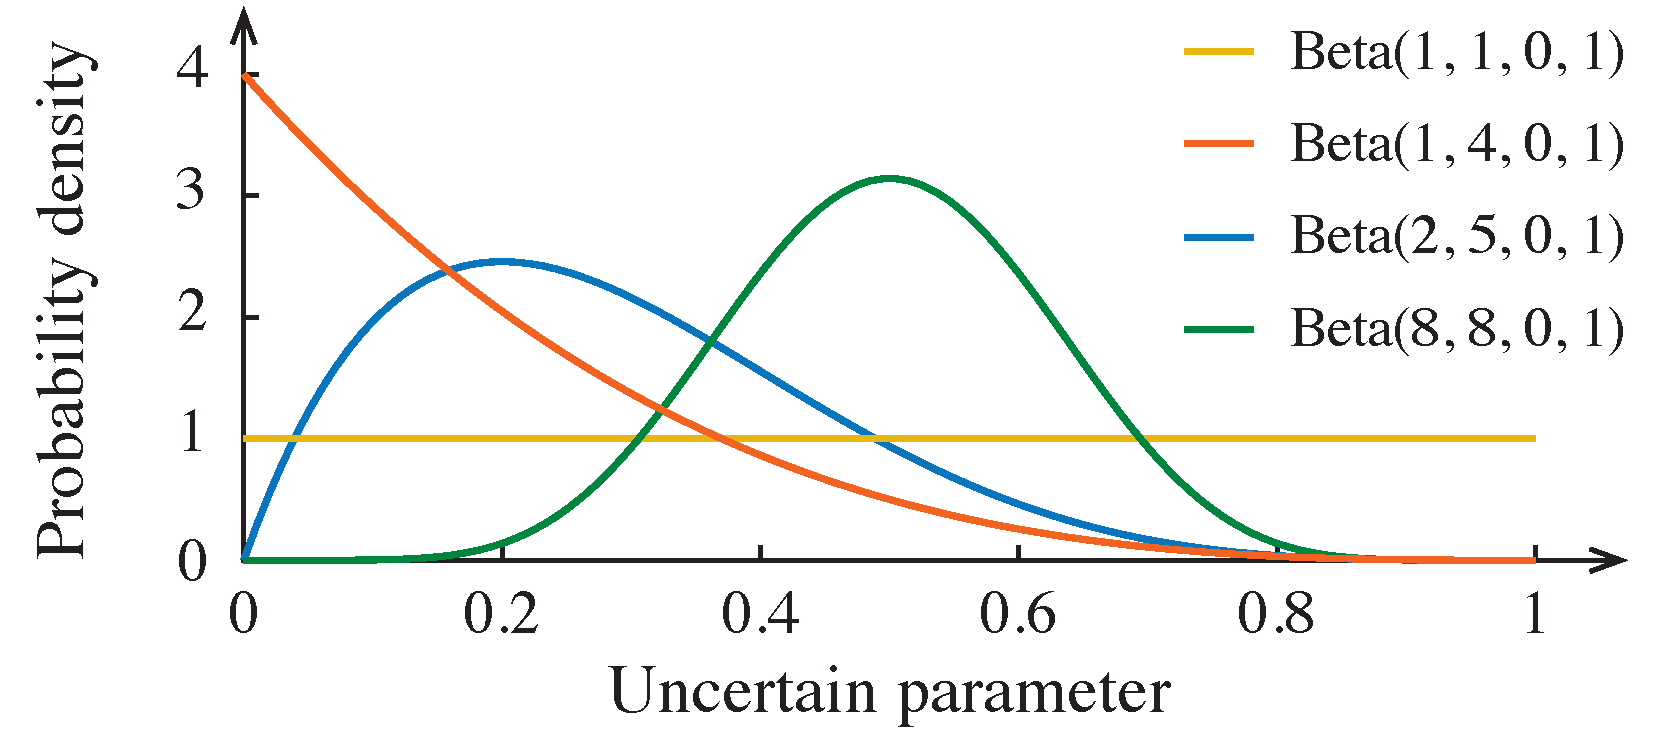
\includegraphics[width=1.0\columnwidth]{include/assets/figures/distribution.pdf}
  \caption{An illustration of the family of beta distributions.}
  \flab{distribution}
\end{figure}

The uncertain parameters $\vu$ are the execution times of the tasks; all other
parameters are deterministic. Targeting the practical scenario described in
\sref{parameters}, the marginal distributions and correlation matrix of $\vu$
are assumed to be available. Without loss of generality, the marginal of $\u_i$
is a four-parametric beta distribution $\text{Beta}(\alpha_i, \beta_i, a_i,
b_i)$ where $\alpha_i$ and $\beta_i$ are the shape parameters, and $a_i$ and
$b_i$ are the endpoints of the support. This family of distributions is very
reach; \fref{distribution} illustrates how the density function changes
dramatically depending on $\alpha_i$ and $\beta_i$. The left $a_i$ and right
$b_i$ endpoint are set to 80\% and 120\%, respectively, of the reference
execution time generated by the \up{TGFF} tool as described earlier. The
parameters $\alpha_i$ and $\beta_i$ are set to two and five, respectively, for
all tasks, which skews the corresponding distribution toward the left endpoint
as shown in \fref{distribution}. The execution times of the tasks are correlated
based on the structure of the graph produced by the \up{TGFF} tool: the closer
task $i$ and task $j$ are in the graph as measured by the number of edges
between vertex $i$ and vertex $j$, the stronger $\u_i$ and $\u_j$ are
correlated. The model-order reduction parameter $\eta$ in \eref{reduction}
(\sref{parameters}) is set to 0.95, which results in $\nz = 2$ and 3 independent
variables for applications with $\nt = 10$ and 20 tasks, respectively.

The configuration of the interpolation algorithm (the collocation nodes, basis
functions, and adaptivity strategy with stopping conditions) is as described in
\sref{interpolation}. The parameters $\aerror$, $\rerror$, and $\serror$ vary
depending on the problem and can be found at \cite{sources}, which, again,
contains all other details too.

The performance of our framework with respect to each problem is assessed as
follows. First, we obtain the ``true'' distribution of the quantity in question
$\g$ by sampling $\g$ directly and extensively. Direct sampling means that $\g$
is evaluated \emph{as is}; in particular, no model-order reduction is perform,
which could affect the resulting accuracy (see \sref{parameters}). Second, we
construct an interpolant for $\g$ and estimate $\g$'s distribution by sampling
the interpolant. In both cases, we draw $10^5$ samples; let us remind, however,
that the cost of sampling the interpolant is practically zero. Third, we perform
another round of direct sampling of $\g$, but this time we draw as many samples
as many times the quantity was evaluated during the interpolation process. In
each of the three cases, the sampling is undertaken in accordance with a Sobol
sequence, which is a quasi-random low-discrepancy sequence featuring much better
convergence properties than those of the vanilla Monte-Carlo sampling
\cite{joe2008}.

As a result, we obtain three estimates of $\g$'s distribution: reference (the
one considered true), interpolation powered (the one proposed), and na\"{i}ve
(the one direct and equal in terms of the number of $\g$'s evaluations to the
proposed solution). The last two are compared with the first one. For comparing
the proximity between two distributions, we use the well-known
Kolmogorov--Smirnov statistic \cite{rao2009}, which is the supremum over the
distance between two empirical distribution functions and, hence, is a rather
unforgiving error indicator.

\begin{figure*}
  \vspace{-1.5em}
  \centering
  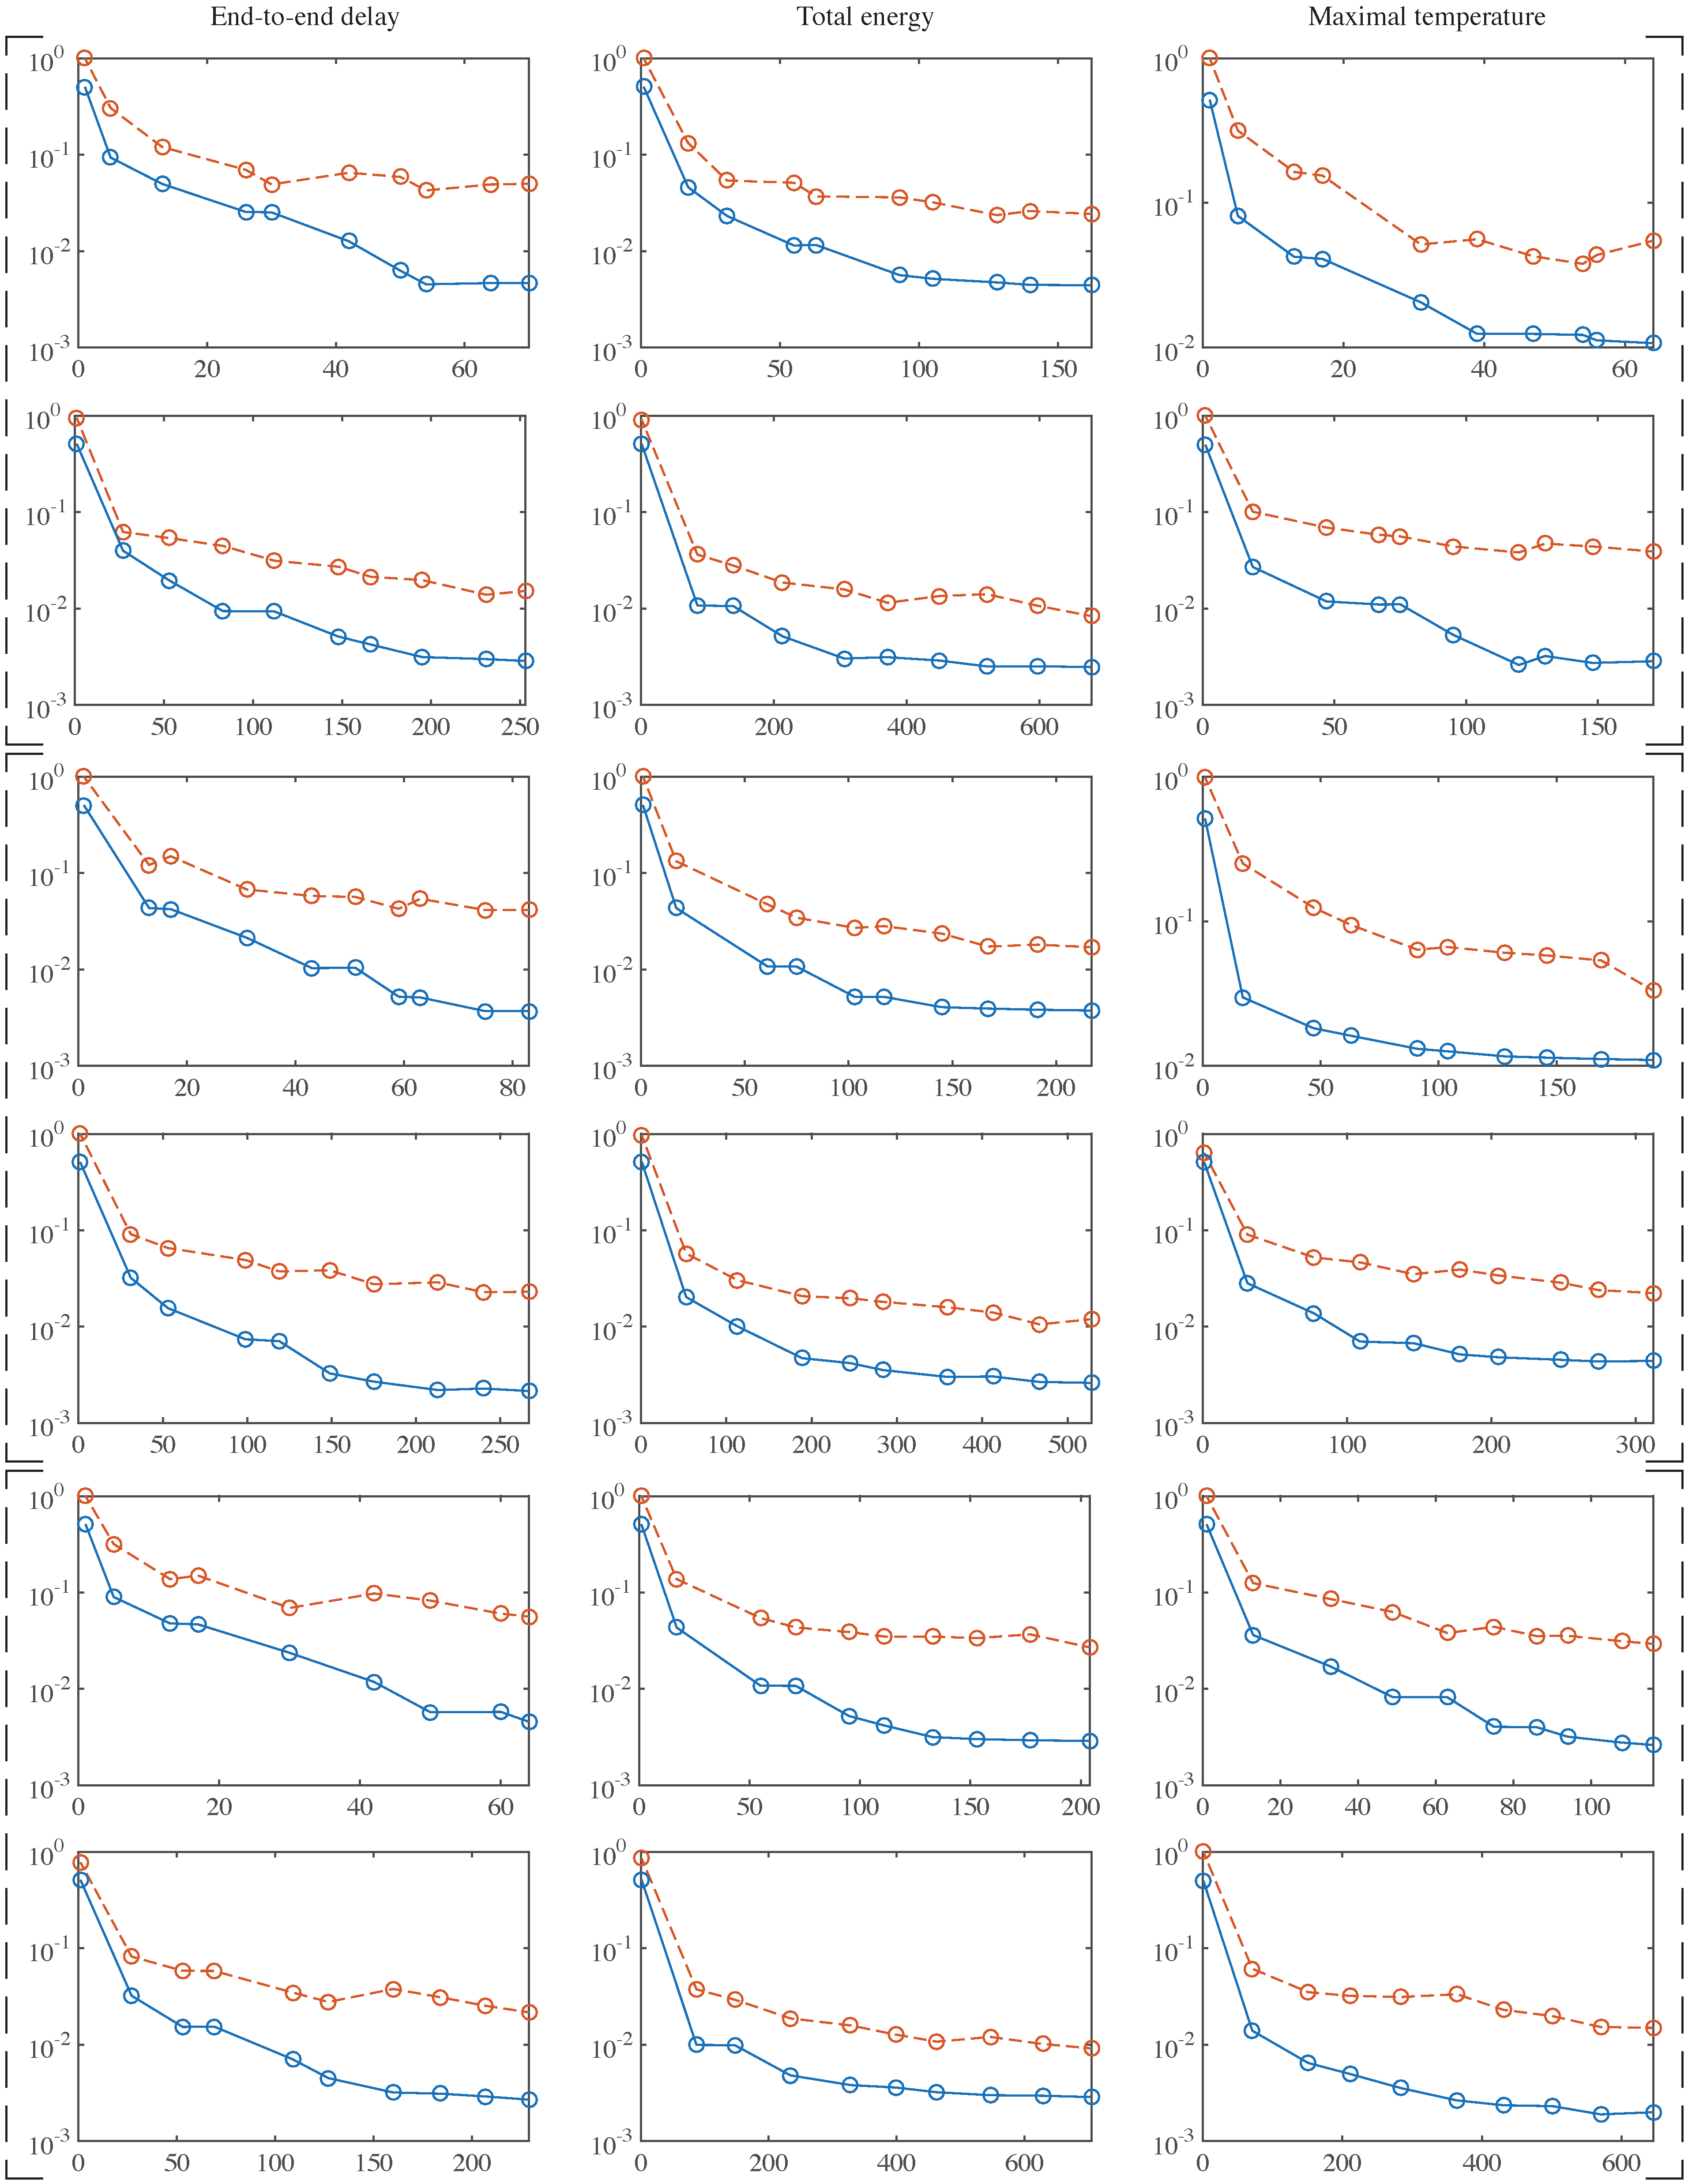
\includegraphics[width=1.0\textwidth]{include/assets/figures/results.pdf}
  \vspace{-1.5em}
  \caption{
    Experimental results. There are considered 3 quantities, 3 platform sizes,
    and 2 application sizes. The columns correspond to the three quantities: the
    end-to-end delay (left), total energy (middle), and maximum temperature
    (right). The three pairs of rows correspond to the three platform sizes: 2
    (top), 4 (middle), and 8 (bottom) processing elements. The rows alternate
    between the two application sizes: 10 (odd) and 20 (even) tasks. The
    horizontal axes show the number of points, and the vertical ones the error
    on a logarithmic scale. The solid lines correspond to our technique, and the
    dashed ones to direct sampling.
  }
  \flab{results}
\end{figure*}

\subsection{Discussion}
The results for all 18 experiments are given in \fref{results}.

Let $\g$ be the end-to-end delay given by \eref{end-to-end-delay}.

Let $\g$ be the total energy given by \eref{total-energy}.

Let $\g$ be the maximum temperature given by \eref{maximum-temperature}.
